\section{Buổi 1}

\textbf{Khoa học dữ liệu thị giác là gì?}

\textbf{Câu 1: Giải thích về cách mạng công nghiệp chuyển đổi số và cho ví dụ}\\
Đây là giai đoạn mà công nghệ số được tích hợp sâu vào mọi lĩnh vực kinh tế và xã hội, làm thay đổi cách con người sản xuất, quản lý và sinh hoạt. Chuyển đổi số không chỉ là đưa máy tính hay Internet vào sử dụng, mà là:

\begin{itemize}
	\item Chuyển dữ liệu và quy trình sang dạng số
	
	\item Kết nối con người, máy móc và hệ thống
	
	\item Ra quyết định dựa trên dữ liệu và tự động hóa
\end{itemize}

Thay vì ngày xưa phải đi đến trực tiếp cửa hàng thì mới mua được hàng, phải đến trực tiếp quán ăn mới ăn được thì bây giờ mọi người có thể đặt giao hàng trực tuyến qua các ứng dụng, sau đó sẽ có các nhân viên giao đến tận nơi giúp mình.

Lúc trước, muốn thực hiện một giao dịch ngân hàng hay những hoạt động về tài chính thì phải đến trực tiếp ngân hàng thì mới thực hiện được. Nhưng bây giờ ta có thể thực hiện hoàn toàn trực tuyến, một cách nhanh chóng và tiện lợi thông qua các ứng dụng banking của ngân hàng.

\textbf{Giải thích "Thông minh hoá \textbf{qui trình sản xuất} và \textbf{quản lý xã hội} trên thế giới ở diện rộng với \textbf{nền tảng chuyển đổi số}, trong đó \textbf{AI}giữ vai trò cốt lõi}

\textbf{Các ví dụ về chuyển đổi số}

\textbf{Bốn cuộc cách mạng công nghiệp}

\textbf{Câu 6: Nêu điểm khác biệt của mắt người và thiết bị số khi thu thập hình ảnh}

\begin{table}[H]
	\centering
	\begin{tabular}{|p{7cm}|p{7cm}|}
		\hline
		Mắt người & Thiết bị số \\ \hline
		Thu nhận ánh sáng bằng võng mạc & Thu nhận ánh sáng bằng cảm biến CCD hoặc CMOS \\ \hline
		Xử lý hình ảnh kết hợp sinh lý và nhận thức của não & Xử lý theo thuật toán \\ \hline
		Độ phân giải thay đổi theo vùng nhìn & Độ phân giải cố định theo số lượng pixel \\ \hline
		Vùng trung tâm nhìn rõ hơn vùng ngoại vi & Phân bố đồng đều trên toàn ảnh \\ \hline
		Thích nghi tốt với thay đổi ánh sáng & Phụ thuộc cảm biến và thuật toán xử lý \\ \hline
		Ghi nhớ chọn lọc và mang tính nhận thức & Dễ sao chép và xử lý \\ \hline
	\end{tabular}
\end{table}

\textbf{Các đặc trưng khi tiếp nhận một bức ảnh}

\textbf{Câu 5: Thách thức về lỗ hổng ngữ nghĩa của hệ thống thị giác là gì?}

Thách thức về lỗ hổng ngữ nghĩa (semantic gaps) trong hệ thống thị giác máy tính là một trong những thách thức lớn nhất mà các hệ thống thị giác máy tính phải đối mặt. Chẳng hạn như:

\begin{itemize}
	\item Hệ thống xử lý hình ảnh ở mức pixel, các giá trị số hoặc đặc trưng kỹ thuật, mà bản thân chúng không mang ý nghĩa ngữ nghĩa rõ ràng.
	
	\item Hệ thống có thể không hiểu được rõ hết được ngữ nghĩa mà con người muốn, chẳng hạn như "đây là một con mèo đang ngủ trên ghế".
	
	\item Ngoài ra ý nghĩa của một đối tượng trong hình ảnh còn phụ thuộc vào ngữ cảnh xung quanh. Ví dụ: Một con dao có thể là dụng cụ nhà bếp hoặc một vật nguy hiểm, tùy thuộc vào môi trường (nhà bếp hoặc một cảnh hành động).
	
	\item Một đối tượng hoặc cảnh có thể mang nhiều ý nghĩa khác nhau trong các tình huống khác nhau. Ví dụ: Một biểu cảm khuôn mặt có thể biểu thị niềm vui hoặc sự mỉa mai, tùy thuộc vào bối cảnh.
\end{itemize}

\textbf{Đột phá khi giải quyết được Semantic Gap}

\textbf{Hiện nay, Khoa học dữ liệu thị giác đã giải quyết Semantic Gap như thế nào?}

\textbf{Các ví dụ cần đến lĩnh vực}

\textbf{Câu 8: Phân biệt Computer Graphic, Image \& Video Processing và Computer Vision}

\begin{table}[H]
	\centering
	\begin{tabular}{|c|p{4cm}|p{4cm}|p{4cm}|}
		\hline
		& Computer Graphics & Image \& Video Processing & Computer Vision \\ \hline
		Mục tiêu & Mô phỏng thế giới thực và thế giới ảo & Tăng cường chất lượng ảnh/video & Tăng cường khả năng hiểu ảnh/video cho máy tính \\ \hline
		Input & Điểm 2D, 3D, các loại đường cong & Ảnh/video & Ảnh/video \\ \hline
		Output & Các thực thể hình học 2D, 3D & Ảnh/video tăng cường & Ngữ nghĩa của ảnh/video \\ \hline
	\end{tabular}
\end{table}

\section{Buổi 2}

\textbf{Detect Bounding Box cho người, vật để làm gì?}

\textbf{Câu 2: Thế nào là thông minh?}

Thông minh là khả năng thích ứng của sự thay đổi hay nói một cách khác là khả năng nắm bắt bản chất của sự vật hiện tượng một cách nhanh chóng.

\textbf{Phân biệt trí tuệ nhân tạo và trí tuệ tự nhiên (Bảng: cơ chế, năng lượng, bộ nhớ, khả năng sáng tạo)}

\textbf{Con người nghĩ ra Trí tuệ nhân tạo thì sáng tạo ở điểm nào}

\textbf{Khuyết điểm của Trí tuệ nhân tạo so với con người trong việc sáng tạo}

\textbf{Trí tuệ nhân tạo có gì đặc biệt so với trí tuệ con người}

\textbf{Trí tuệ tự nhiên kém điểm nào}

\textbf{Giải thích câu nói "I’m intrigued that AI has by now succeeded in doing essentially everything that requires “thinking” but has failed to do most of what people and animals do “without thinking”" của Donald Knuth}

\textbf{Câu 3: Giải thích câu nói “Intelligence is the ability to adapt to change." - Stephen Hawking}

Câu nói "Intelligence is the ability to adapt to change." của Stephen Hawking nhấn mạnh rằng trí thông minh không chỉ đơn thuần là kiến thức hay kỹ năng cố định, mà còn là khả năng linh hoạt, thích ứng với những thay đổi không ngừng của môi trường xung quanh.

\textbf{Học máy là gì? Học máy có gì khác với học thông thường?}

\textbf{Ví dụ cho việc càng sử dụng mô hình, mô hình càng cải thiện}

\textbf{Học sâu là gì?}

\textbf{Vì sao xảy ra hiện tượng blackbox nhưng con người vẫn tin tưởng vào output?}

\textbf{Huấn luyện ChatGPT đã sử dụng bao nhiêu GPU (loại nào)?}

\textbf{Reinforce Learning được ứng dụng nhiều ở đâu}

\textbf{Ví dụ cho output của hệ thống thị giác theo 5 cấp độ - Mức độ thông mình của đầu ra của hệ thống thị giác}

\section{Buổi 3}

\textbf{Tên các phần mềm đồ hoạ liên quan đến}

\textbf{Vì sao con người nhìn được nhiều màu?}

Mắt người có các tế bào thụ cảm ánh sáng gọi là tế bào nón (cones). Có 3 loại tế bào nón chính, mỗi loại nhạy cảm với một dải bước sóng ánh sáng khác nhau:

\begin{itemize}
	\item \textbf{L-cones:} Nhạy với bước sóng dài (màu Đỏ).
	
	\item \textbf{M-cones:} Nhạy với bước sóng trung bình (màu Xanh lá).
	
	\item \textbf{S-cones:} Nhạy với bước sóng ngắn (màu Xanh dương).
\end{itemize}

Màu sắc trên một vật xuất hiện nhờ vào cách mà vật thể tương tác với ánh sáng. Khi ánh sáng chiếu vào bề mặt của một vật thể, vật đó sẽ hấp thụ các bước sóng nhất định và phản xạ các bước sóng khác. Các bước sóng phát ra sau đó truyền tới mắt chúng ta, các tế bào nón kết hợp chúng lại để tạo ra cảm giác về màu sắc.

\textbf{Vì sao trong in ấn sử dụng CMYK nhưng màn hình lại sử dụng RGB}

Vì não bộ chúng ta tạo ra cảm giác về màu sắc bằng cách kết hợp tín hiệu từ 3 loại tế bào nón, nên các kỹ sư chỉ cần sử dụng 3 nguồn sáng tương ứng (Red, Green, Blue) cùng nguyên lý cộng màu để "đánh lừa" mắt rằng chúng ta đang thấy hàng triệu màu sắc khác nhau.

\begin{itemize}
	\item Mỗi điểm ảnh (pixel) trên màn hình thực chất gồm 3 điểm màu siêu nhỏ: Đỏ, Xanh lá và Xanh dương.
	
	\item Khi trộn các luồng ánh sáng này với cường độ khác nhau, chúng tạo ra các màu mới. Ví dụ: Đỏ + Xanh lá = Vàng; Đỏ + Xanh lá + Xanh dương = Trắng.
	
	\item Với 3 thành phần này, chúng ta có thể tạo ra một dải màu (gamut) đủ rộng để đáp ứng hầu hết nhu cầu quan sát của con người.
\end{itemize}

Tuy nhiên, trong in ấn, người ta lại dùng 4 thành phần (CMYK: Cyan, Magenta, Yellow, Black). Điều này là do mực in hoạt động theo nguyên lý trừ màu (hấp thụ ánh sáng) thay vì phát sáng, nên cần thêm màu đen (K) để tạo độ tương phản sâu mà 3 màu kia khi trộn lại khó đạt được một cách hoàn hảo.

\textbf{Trình bày cách tính toạ độ chiếu (u, v) dựa vào toạ độ thực (x, y, z) và tiêu cự f (khoảng cách tâm chiếu)}

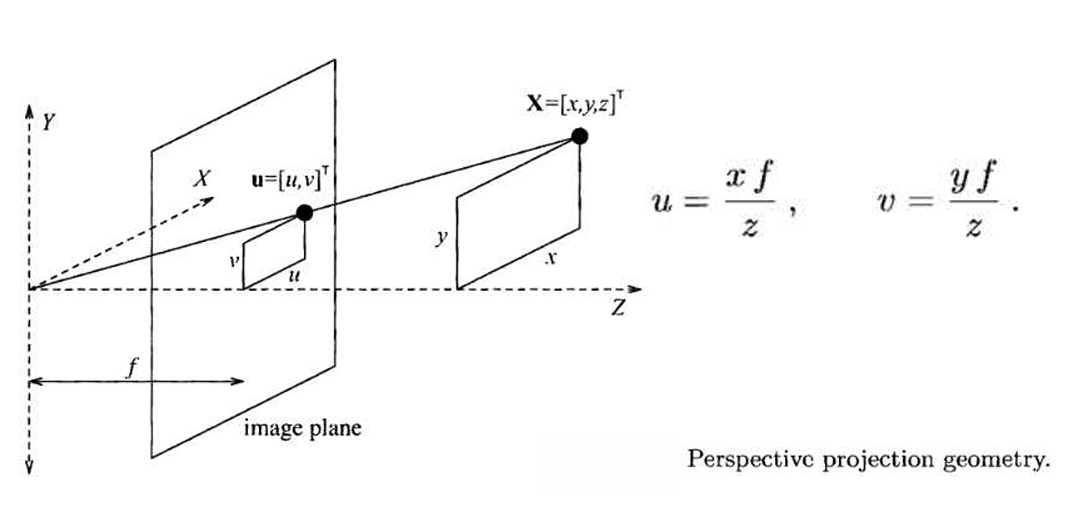
\includegraphics[width=\linewidth]{perspective.png}

\section{Buổi 4}

\textbf{Giải thích, cho ví dụ về H, S, V trong hệ màu HSV}

Không gian màu HSV (Hue, Saturation, Value) là một hệ màu được sử dụng để tạo ra tất cả các màu thông qua ba thông số chính: Hue (H) biểu thị sắc màu, Saturation (S) thể hiện độ bão hòa của màu sắc, và Value (V) chỉ mức độ sáng của màu. Trong đó:

\begin{itemize}
	\item Hue xác định bản chất của màu sắc mà không phụ thuộc vào độ sáng hoặc độ bão hòa, ví dụ như Đỏ, Xanh, Vàng.
	
	\item Saturation càng cao, màu sắc càng rực rỡ và mạnh mẽ. Saturation thấp làm màu sắc trở nên nhợt nhạt, gần như chỉ còn là tông xám, ví dụ như độ tươi của màu: đỏ tươi, đỏ đô.
	
	\item Value quyết định xem màu sắc đó trông sáng, tối, hoặc gần như đen.
\end{itemize}

\textbf{Trong thế giới có bao nhiêu đối tượng 2D, 3D}

\textbf{Thực thể cơ bản trong 3D là gì}

\textbf{Vì sao màn hình nhỏ có thể mô phỏng thế giới thực}

\textbf{Trong công thức vẽ đoạn thẳng $p_0 = 2 \Delta y - \Delta x$, $\Delta x$, $\Delta y$ là gì?}

\textbf{Giải thích (khuyết điểm) giải thuật DDA của vẽ đoạn thẳng}

\textbf{Nguyên lý vẽ đoạn thẳng}

\textbf{Bài tập: Vẽ đoạn thẳng qua A(20; 10), B(30; 18)}

\textbf{Chứng minh trong góc 1/8, |hệ số góc tiếp tuyến| < 1}

\textbf{Chứng minh: nếu điểm giữa thuộc miền trong chọn $y_k$ (<=> $p_k < 0$), nếu điểm giữa thuộc miền ngoài -> chọn $y_k - 1$ (<=> $p_k > 0$)}

\textbf{Tính $p_0$ trong công thức quy nạp đường tròn}

\textbf{Chứng minh với r nguyên, có thể dùng $p_0' = p_0 - \frac{1}{4}$ mà các công thức vẫn đúng}

\textbf{Bài tập: Vẽ đường tròn tâm O(0; 0), bán kính r = 10}

\textbf{Giải thích ý nghĩa góc $\varphi$ trong phương trình ellipse trong hệ toạ độ cực}

\textbf{Bài tập: Vẽ ellipse tâm O(0; 0), $r_x = 8$, $r_y = 6$}

\section{Buổi 5}

\textbf{Chứng minh: Đường cong Bezier đi qua 2 điểm đầu mút}

\textbf{Chứng minh: Đường cong Bezier tiếp xúc với 2 đoạn điều khiển tại 2 đầu mút}

\textbf{Tính đạo hàm bậc 2}

\textbf{Nếu có các tính chất như thế thì có lợi gì?}

\textbf{So sánh đường cong Spline Hermite với đường cong Bezier bậc 3}

\textbf{Sau khi thay đổi 1 trong các điểm điều khiển thì đường cong bị sửa đổi toàn cục hay cục bộ? Vì sao?}

\textbf{Chứng minh tại điểm kết nối đạt $C^0$, $C^1$}

\textbf{Giải thích ý nghĩa của tính chất bất biến affine}

\section{Buổi 6}

\textbf{Khuyết điểm tô màu theo vết mực loang (Boundary Fill)}
Độ phức tạp tính toán chậm,

\textbf{Nếu màu biên trùng màu tô thì sao?}

\textbf{Vì sao lại chọn lấp đầy các pixel giữa cặp đỉnh chẵn lẻ?}

\textbf{Có trường hợp nào phương pháp tô màu theo dòng quyết gặp khó khăn?}
Đi qua đỉnh, đi qua cạnh song song

\textbf{Tiêu chí chọn đỉnh để làm ngắn cạnh}

\textbf{Đề xuất cấu trúc dữ liệu AEL cho phương pháp tô màu theo dòng quét}

\section{Buổi 7}

\textbf{Định nghĩa 3 cấu trúc bảng cho đối tượng 3 chiều}

\textbf{Xây dựng hàm sinh tập đỉnh, cạnh, mặt dựa trên phương trình cầu trong hệ toạ độ cực}

\textbf{Viết phương trình TabSurf}

\textbf{Giải thuật xây dựng TabSurf}

\textbf{Ví dụ của TabSurf trong thực tế}

\textbf{Vẽ mặt yên ngựa bằng CoonsSurf}

\textbf{Viết phương trình Revolution Surf}

\textbf{Giải thuật xây dựng Revolution Surf}

\section{Buổi 8}

\textbf{Xây dựng chương trình chiếu quả cầu (chỉ chiếu các đỉnh) lên 2D}

\textbf{Xây dựng ma trận phép quay quanh 1 trục bất kỳ}

\textbf{Nếu mắt người chiếu song song thay vì chiếu phối cảnh thì gặp trở ngại gì?}






































































